\documentclass[a4paper]{article}
\usepackage[parfill]{parskip} % For line skip paragraphs
\usepackage[utf8]{inputenc}
\usepackage{geometry}
\usepackage{fancyhdr}
\usepackage[pdftex]{graphicx}
\usepackage{cite}
\usepackage{listings}
\usepackage{caption}
\usepackage{color}
\usepackage{underscore}
\usepackage{url}

\usepackage{courier}

% from http://stackoverflow.com/questions/741985/latex-source-code-listing-like-in-professional-books
 \lstset{
         basicstyle=\footnotesize\ttfamily, % Standardschrift
         numbers=left,               % Ort der Zeilennummern
         numberstyle=\tiny,          % Stil der Zeilennummern
         %stepnumber=2,               % Abstand zwischen den Zeilennummern
         numbersep=5pt,              % Abstand der Nummern zum Text
         tabsize=2,                  % Groesse von Tabs
         extendedchars=true,         %
         breaklines=true,            % Zeilen werden Umgebrochen
         keywordstyle=\color{red},
            frame=b,         
%        keywordstyle=[1]\textbf,    % Stil der Keywords
%        keywordstyle=[2]\textbf,    %
%        keywordstyle=[3]\textbf,    %
%        keywordstyle=[4]\textbf,   \sqrt{\sqrt{}} %
         stringstyle=\color{white}\ttfamily, % Farbe der String
         showspaces=false,           % Leerzeichen anzeigen ?
         showtabs=false,             % Tabs anzeigen ?
         xleftmargin=17pt,
         framexleftmargin=17pt,
         framexrightmargin=5pt,
         framexbottommargin=4pt,
%         showstringspaces=false      % Leerzeichen in Strings anzeigen ?        
 }

\DeclareCaptionFont{white}{ \color{white} }
\DeclareCaptionFormat{listing}{
  \colorbox[cmyk]{0.43, 0.35, 0.35,0.01 }{
    \parbox{\textwidth}{\hspace{15pt}#1#2#3}
  }
}
\captionsetup[lstlisting]{ format=listing, labelfont=white, textfont=white, singlelinecheck=false, margin=0pt, font={bf,footnotesize} }

%TCIDATA{OutputFilter=LATEX.DLL}
%TCIDATA{Version=5.50.0.2953}
%TCIDATA{<META NAME="SaveForMode" CONTENT="1">}
%TCIDATA{BibliographyScheme=Manual}
%TCIDATA{Created=Monday, January 30, 2012 17:20:46}
%TCIDATA{LastRevised=Monday, February 27, 2012 12:06:08}
%TCIDATA{<META NAME="GraphicsSave" CONTENT="32">}
%TCIDATA{<META NAME="DocumentShell" CONTENT="Standard LaTeX\Blank - Standard LaTeX Article">}
%TCIDATA{CSTFile=40 LaTeX article.cst}

\newenvironment{proof}[1][Proof]{\noindent\textbf{#1.} }{\ \rule{0.5em}{0.5em}}

% Sets page margins to 1", which is standard
%\geometry{left=1in,right=1in,top=1in,bottom=1in} 

% allows the included extensions of graphic files
\DeclareGraphicsExtensions{.pdf,.png,.jpg}

% sets/adds graphic path. If empty it just looks around the folder the .tex file is in
\graphicspath{{}}

% I do not remember what this does
\setlength{\headheight}{15.2pt}

% allows the xhead parameters
\pagestyle{fancy}

% Sets the left header
\lhead{Bye, Gombos \& Lundal}

% Sets the right header
\rhead{Exercise 2, TDT4255 Autumn 2013}

% everything before this is considered the header or whatever.
\begin{document}

% INCLUDEGRAPHICS EXPLANATION
% \includegraphics[scale=1]{name of file}
% sometimes you want to twice encase the filename in squiggly brackets. I do not know why but sometimes it is required.

% begin title page, use \\ for newline
\title{Report for Exercise 2\\Optimized Pipelined MIPS Processor\\\vspace{2mm}\Large{TDT4255 Computer Design}}

% now one can list the authors, \textbf{} makes bold text
\author{Emil Taylor Bye \and Péter Henrik Gombos \and Per Thomas Lundal}


\pagenumbering{roman}

% make title page
\maketitle


\bigskip
\bigskip
\bigskip
\bigskip

\section*{Abstract}

This report describes the implementation of an Optimized Pipelined processor
with the MIPS instruction set. The processor is tested both on a computer and an
FPGA, and shown to work well.


\clearpage

\tableofcontents

\clearpage

\listoffigures

%\setcounter{secnumdepth}{3}

\clearpage

\setcounter{page}{1}
\pagenumbering{arabic}

\section{Introduction}

\subsection{Pipelining}

Pipelined vs multi-cycle

Pipeline bubbles

\subsection{Optimization}

Forwarding

Branch prediction



\clearpage

\section{Description}

The assignment was to improve the implementation from the previous exercise with
a pipeline instead of the datapath, and implement optimizations that improve the
performance of the processor. This was to be tested on the FPGA onboard a 
MicroBlaze-based embedded system.

\subsection{Requirements}
The processor should include a 5-stage pipeline, and otherwise follow the
requirements from the previous exercise. This includes using a limited MIPS
instruction set.

\subsection{Suggestions}
It was suggested that we followed the architecture presented by Patterson and
Hennessy, as supplied in figure \ref{fig:suggestedArchitecture}.

\begin{figure}[ht]
    \centering
    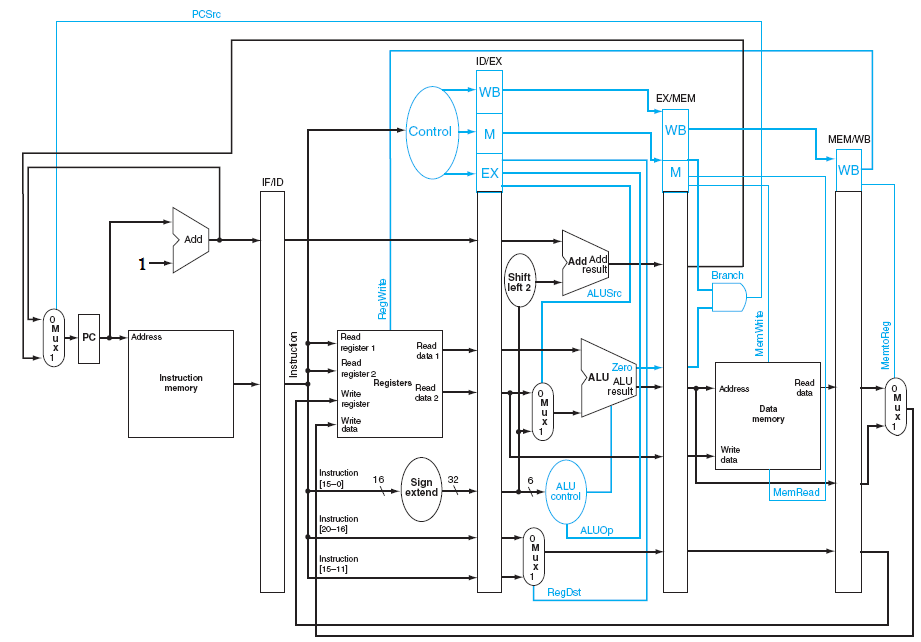
\includegraphics[width=\textwidth]{figures/SuggestedArchitecture.png}
    \caption{The suggested CPU architecture} 
    \label{fig:suggestedArchitecture}
\end{figure}


\subsection{Supplied material}
\begin{itemize}
    \item Communication Framework -  Providing an interface towards the embedded system
    \item VHDL Components - Register File, ALU and Adder
    \item Test Program - For verification of design
    \item main.c - MicroBlaze script for handling communication
    \item host.py - Python script for handling communication
\end{itemize}


\clearpage

\section{Solution}

\subsection{Architecture}

The suggested architecture in figure \ref{fig:suggestedArchitecture} only supports a handful of MIPS instructions. 

\begin{figure}[ht]
    \centering
    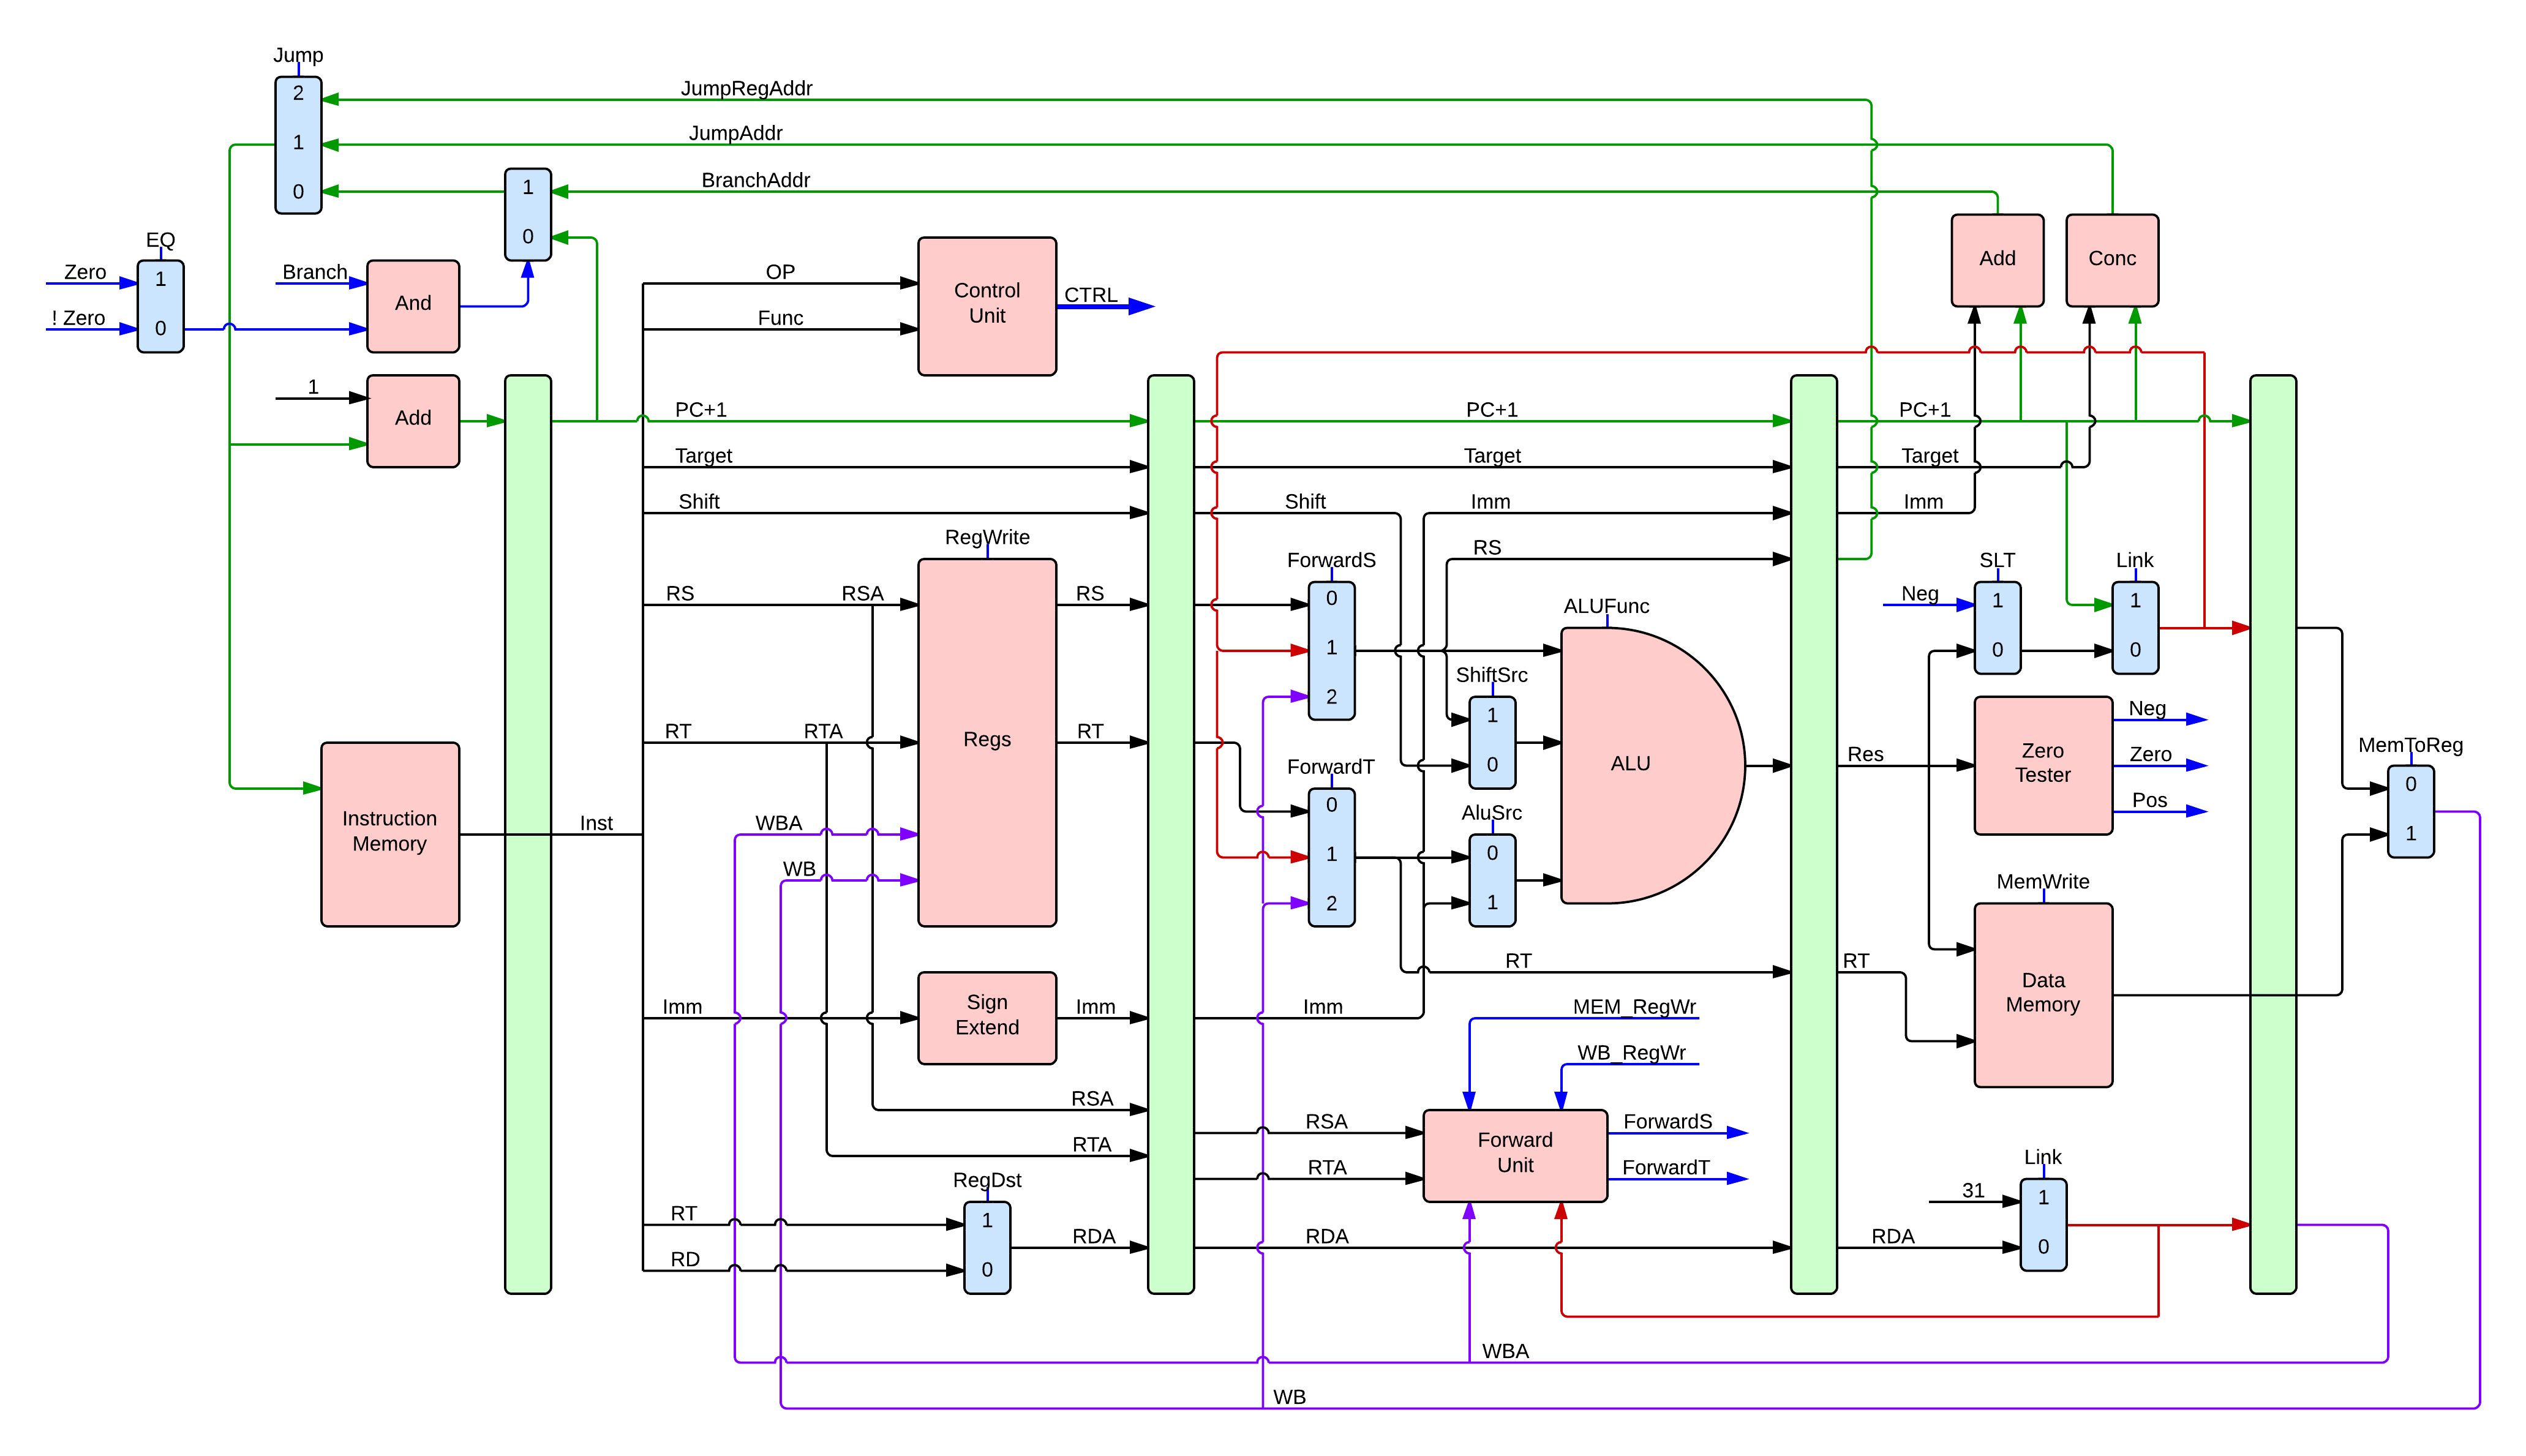
\includegraphics[width=\textwidth]{figures/Architecture.png}
    \caption{\label{fig:cpuArchitecture}The implemented CPU architecture} 
\end{figure}



Output from mems goes right through pipeline registers bc they act on clock tick

\subsection{Instruction Set}

\subsection{Control Unit}


\subsection{Forwarding Unit}

\subsection{Branch Prediction}



\clearpage

\section{Results}

\subsection{Simulation}

The behaviour of the impementation was tested by writing small programs that would try to provoke certain errors and write debug data to the registers.
They programs were written in a simplified assembly variant and then passed through the assembler to produce signals constants which could be pasted directly into tb\_toplevel.vhd.
The simulation was then run, and the resulting data in the registers was compared to the desired data corresponding to the assembly.

Alu operations, memory operations, forwarding, jumping, branching and flushing were all tested and proved to work correctly.
The test programs can be found in section \ref{testprogs} of the appendix, and there are currently no known bugs.

\subsection{Timing Simulation}

\begin{figure}[ht]
    \centering
    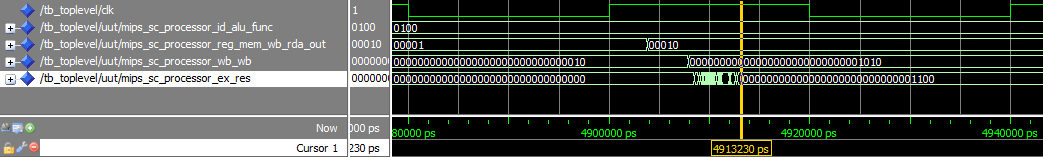
\includegraphics[scale=0.5]{figures/TimingSimulation.png}
    \caption{Timing diagram for critical path} 
    \label{fig:timing}
\end{figure}

Figure \ref{fig:timing} is a timing diagram showing the output from the ALU, which is the end of the critical path that starts at the ex/mem pipeline register and goes through the bottom link mux, the forwarding unit, the forwarding mux, and into the ALU.
The time from a rising clock edge to a the output is stable is shown to be $13.230$ ns, which translates to a maximum clock speed of about $75$ Mhz.
This is very close to the max clock speed of $77.442$ MHz reported by the synthesis tool.

\subsection{Verification}

By following the extensive procedure in the compendium \cite[p.47]{lab-compendium} and using the supplied user\_logic.vhd and main.c files, the design was added to the MicroBlaze framework and compiled to a bit file, before uploading it to an AvNet Development Board by using AvProg.
When the board was ready for input, as seen in figure \ref{fig:avprog}, the test program flush\_test was loaded to the FPGA by using host.py, before running it.
The memory dump in section \ref{memdump} of the appendix confirms that the program executed correctly.

\begin{figure}[ht]
    \centering
    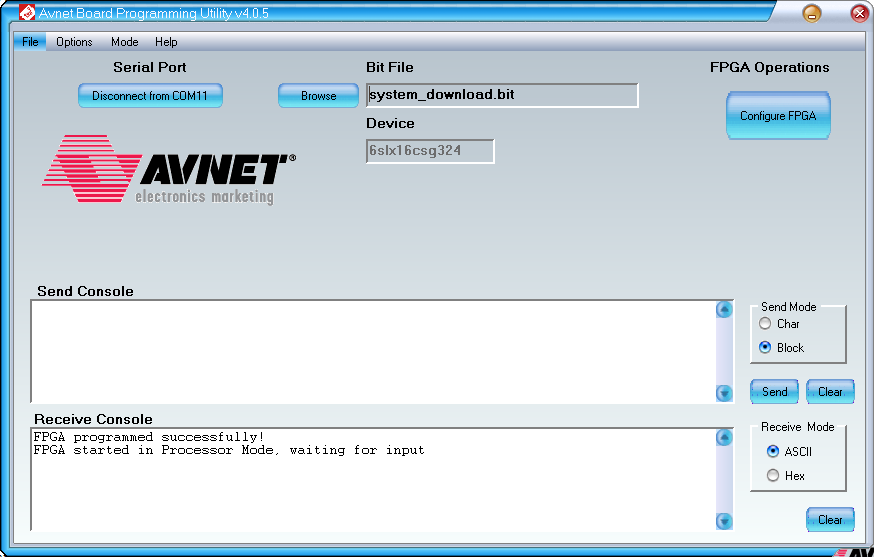
\includegraphics[scale=0.5]{figures/AVNET.png}
    \caption{FPGA programmed successfully} 
    \label{fig:avprog}
\end{figure}



\clearpage

\section{Discussion}

\subsection{Warnings}

There are quite a few warnings that pop up during syntezation of the project, but they are not the result of errors or mistakes in the processor implementation.
All come from the supplied framework, and most complain about memory address lines that are not connected, as the framework uses block ram which takes only 8-bit addresses.

\subsection{Assembler}
Since the programs that would be run on the processor should be in machine code,
it is not easy to write them. For that reason, an assembler was written. It is a
completely naive implementation, and does not give anything extra to the
programmer. 

If the processor would be used in real life, it could be wise to add convenient
instructions and things like labels. Some instructions not implemented in the
hardware, such as multiplication, could also be implemented as a
pseudoinstruction.

\subsection{Further optimization}

\subsubsection*{Branch prediction}
The implementated of branch prediction is fairly simple. To further improve the
performance of the processor, more sofisticated branch predictions should be
used.

For example, it could assume that backwards pointing branches would be taken,
while forward pointing ones will not. Other implementation could be to use a
state to give the prediction some memory, and then easier avoid to miss the
prediction twice in a loop.

\subsection{NOP}

Since the processor has no direct ability to halt the output from the memory blocks, a side effect of sending the output from the instruction memory directly through the first pipeline register is that the processor can only be reliably stopped on nops.
If not, the first instruction will be sent through the pipeline twice.

There are a couple solutions for this.
The first is to rewrite the supplied framework to allow the processor to halt the memory output, which creates a great deal of extra work and might cause bugs in other parts of the framework.
The second is to reset the program counter and flush the pipeline when the processor is stopped, which means that the program can not be resumed.

Since each solution has its own side effects, we decided to simply start all
programs with a NOP instruction.



\clearpage

\bibliography{bibtexlibz}{}
\bibliographystyle{plain}
\nocite{*}
All internet resources were checked on \today.
\end{document}
